\documentclass[main.tex]{subfiles} 
\begin{document}

\section*{Teoretisk bakgrunn}
I utredningen, \emph{NOU 2015:8 Fremtidens skole}, vektlegges fagovergripende kompetanser, dvs. 
for eksempel lesing, skriving, utholdenhet, motivasjon, og å kunne planlegge, 
gjennomføre og vurdere egne læringsprosesser (\citeNP[s. 66]{ludv15}) :
\begin{displayquote}
Utvalget anbefaler at fagovergripende kompetanser vektlegges i fremtidens skole. Siden det  
anbefales å integrere dem i fagene, vil informasjon om elevenes kompetanse i fag være viktig.  
Samtidig vil skoler, skoleeiere og nasjonale myndigheter ha behov for informasjon om elevenes utvikling av 
prioriterte fagovergripende kompetanser, for å kunne bidra til at de vektlegges i opplæringen. 
(Ludvigsen-utvalget 2015)
\end{displayquote}
For å vektleggge fagovergripende kompetanser, er da informasjon om elevenes kompetanse i fag viktig. 
Denne informasjonen kan akkumuleres gjennom bruk av formativ vurdering og summativ vurdering.
Gjennom underveisvurderingen, for eksempel, følges elevenes progresjon i faget over tid, og læreren får informasjon
om oppnådd kompetanse. Hensikten med slik vurdering er å gi et grunnlag for å forbedre og videreutvikle  
kvaliteten på opplæringen (\citeNP[s. 92]{ludv15}).

\begin{figure}[h!]
\centering
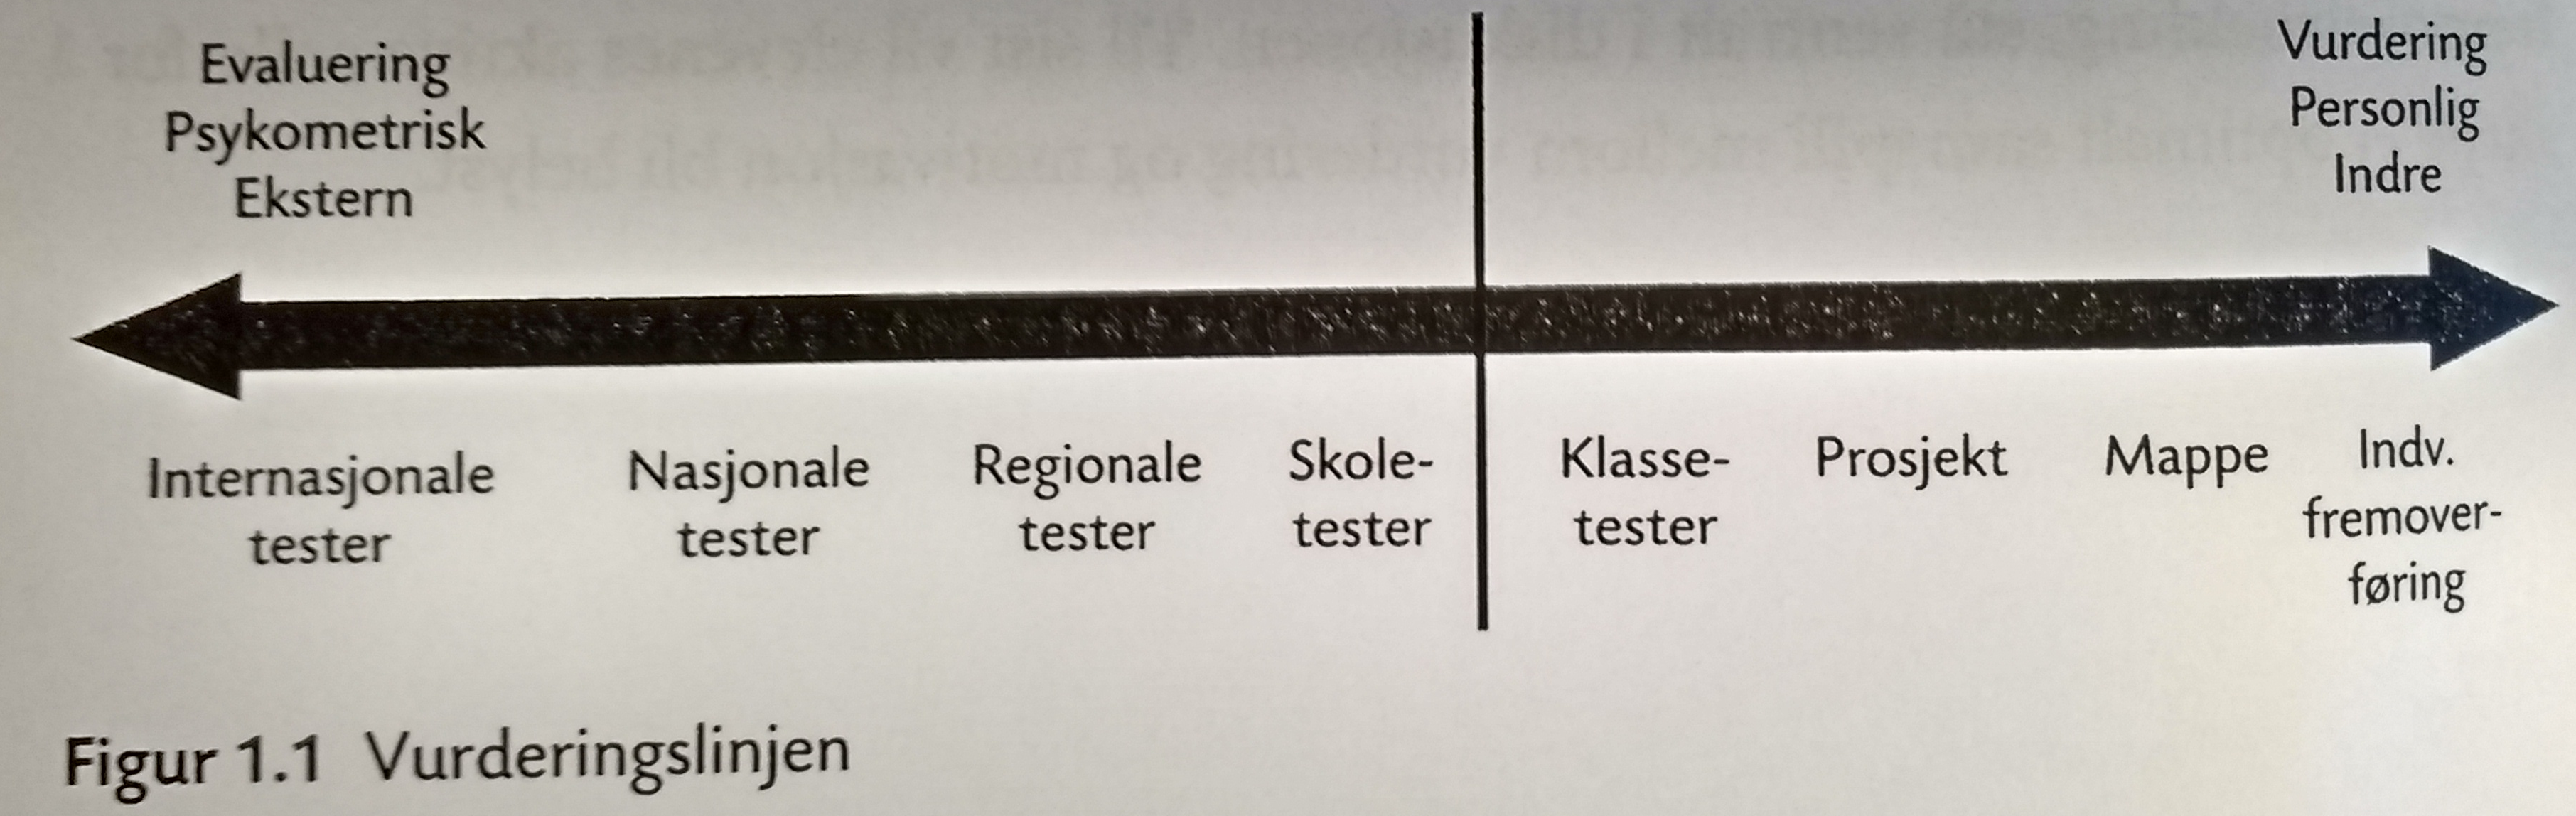
\includegraphics[scale = 0.1]{../figures/vurderingslinjen.png}
\caption{Vurderingslinjen. Kilde: \protect\citeA{smit09}.}
\label{fig:smit09}
\end{figure}


\citeA[s. 3]{smit09} beskriver hvordan vurderingslandskapet forandrer seg, fra internasjonale tester til
individuell fremoverføring. Gjennom \emph{vurderingslinjen} (se figur \ref{fig:smit09}) beskriver hun
hvordan informasjonen går fra å evaluere en nasjon i forhold til andre nasjoner, skoler i distrikter, 
og til slutt på lokalt nivå fra klasser i skolen til enkelt elever i en klasse. Ofte vil politiske styringsorganer
befinne seg på venstre siden av vurderingslinjen, og lærere og elever på høyre siden. Men tiltross for det, 
for undervisere er det viktig å ha oversikt over internasjonale resultater, gjennom f.eks. PISA 
undersøkelsen\footnote{I  PISA-undersøkelsen blir norske 15-åringer sammenliknet med jevnaldrende ungdommer i 
andre OECD-land innen tre sentrale kompetanseområder: matematikk, lesing og naturfag.}. 
Her kan resultatene ha noe å si om hvordan elevenes prestasjoner i ulike fagområder henger sammen med ulike 
bakgrunnsvariabler (\citeNP[s. 11]{klor04}). 

En annen undersøkelse, TIMMS, brukes til evaluere elever helt fra 4.trinn
til andre året på videregående skole. I metastudiet som baserer seg på resultater fra både TIMMS og PISA, 
\citeA{grol06} skriver blant annet at det er interessant å merke forskjellene i resultatene mellom disse to 
studiene. Mens PISA fokuserer på oppgaver rettet nærmere mot virkeligheten, med tabeller og figurer tatt fra virkelige
kontekster, har TIMMS større fokus på ren matematikk. Studiet konkluderer med, for at elevene skal gjøre det bedre
i anvendt matematikk, trenger de en solid fundament i grunnleggende ferdigheter, deriblant tall og tallforståelse.

For eleven derimot er det endatil viktigere å ha informasjon om egen læringsprosess, og denne informasjonen er kritisk 
for en lærer for å vurdere sin egen undervisningspraksis. I læringsrettet vurdering stilles det strengere krav til 
lærerers evner som evaluator. Da er det viktig å se på lærerens læringssyn. Her er følger to eksempeler på 
forskjellige læringssyn.

\subsection*{Læring som overføring av kunnskap}

I behavioristisk læringsteori foregår læring ved overføring av kunnskap, uavhengig av relasjonen mellom lærer 
og elev. Elev blir anskuet som et tomt kar, som det er lærerens jobb å fylle med kunnsakp. 
I et slikt læringssyn er vurdering i seg selv relativt ukomplisert, siden da gjelder det å 
formulere sine tilbakemeldinger på en så presis og elevtilpasset måte som mulig.
Derimot forventes det da at eleven tar til seg tilbakemeldingene og bruker dem til å rette seg etter.
Tilbakemeldingene vil da være begrenset til spesifikke svakheter relatert til faget eller kompetansemål.
Sentralt i behaviorismens syn på læring er betinging (\citeNP[s. 74]{salj13}). Ved ønsket atferd belønnes 
handlingen. Dette referes som forsterking (\citeNP[s. 22]{hell07}). Innenfor vurderingskontekten er
tilsiktet hensikt å motivere elevene. Dermed er karakteren en forsterker for noen og straff for andre.
\newline

Så hva er problemet med en behavioristisk tilnærming til vurdering for læring? La oss tenke at klasserom er 
et sted hvor alle elever er tilnærmet like i hvordan de oppfatter matematikk og hvor deres vanskeligheter ligger. 
Da er det selvfølgelig helt kurant å lage tydelige skriftlige tilbakemeldinger og fremovermeldinger, i et format 
som passer for hele klassen. Dessverre så finnes det ikke slike klasserom, med mindre elever er oppdelt etter nivå. 
Problemmet her er at det strider mot det overordnede prinsippet tilpasset opplæring (\citeNP[s. ]{foss14}). 
\citeA{foss14} kaller dette for organisatorisk differensiering. Fosse referer til Hattie når hun skriver at de flinke 
elevene kan dra nytte av organisaorisk differensiert undervisning, men det har ikke ønsket effekt for elever som strever 
med faget (\citeNP[s. ]{foss14}). Til vanlig skal organiseringen ikke skje etter
faglig nivå, kjønn eller etnisk tilhørlighet. Ifølge opplæringsloven skal alle elever få en opplæring tilpasset 
etter deres evner og forutsetninger. Et annet problem med en slik tilnærming er at elevens deltagelse i egen utvikling 
blir fraværende i et slikt rigid system. Siden eleven er kun en mottager, kan eleven ikke være med og aktivt delta i 
egen vurdering. 

\subsection*{Læring som en relasjonell prosess}

Sett fra det relasjonelle perspektivet består det i å veilede elevene i den nærmeste utviklingssonen.
Den \emph{nærmeste utviklingssonen} beskriver en sone som ligger i mellom en elevs kognitive 
ferdigheter, dvs. hva de kan oppnå selvstendig uten hjelp, og elevens potensielle utvikling, dvs. 
hva en elev kan få til eller forstå gjennom veiledning (\citeNP[s. 125]{bta98}; \citeNP[s. 75]{salj13}). 
Bruk av ''scaffolding`` eller stillasbygging (\citeNP{bta98}) er da viktig for å knytte fagbegreper og teori til elevenes 
forkunnskaper. Vurderingsarbeidet vil derfor også gi den forskende lærer (\citeNP[s. 19]{hell07}) verdifull informasjon 
om sin egen didaktiske tilrettelegging.
Jeg vil komme tilbake til disse læringssyn når jeg evaluerer min egen praksis gjennom FoU arbeidet.
\newline

En av sentrale styringsrammene for norske utdanningspolitikk og skolepraksis er prinsippet om tilpasset opplæring.
Opplæringen skal ivareta sentrale verdier som inkludering, variasjon, sammenheng, relevans, verdsetting, medvirkning og 
erfaringer. Dette skal operasjonaliseres av undervisere gjennom differensiering.  Undervisningen må, ved hjelp av 
differensiering, tilfredsstille alle elevenes tilretteleggingsbehov i klassen, fra elever med matematikkvansker 
(dyskalkuli) til evnerike elever. Når en lærer jobber med elever hvor spennet er så pass stort, med andre ord at elevene 
utgjør en heterogen gruppe, da kan heller ikke undervisningen være homogenisert. Jeg kan derfor allerede nå påstå at en 
behavioristisk tilnærming til vurdering for læring vil tydeligvis ikke oppfylle prinsippet om tilpasset opplæring.

\subsection*{Kartleggingsprøven i sannsynlighetsregning}
Kartleggingsprøver kan brukes i mange forskjellige situasjoner. Ifølge \citeA[s. 15]{brek02} kan diagnostiske oppgaver 
bli brukt til å identifisere og fremheve misoppfatninger som elevene har utviklet, gi læreren informasjon
om elevenes løsningsstrategier og måle hvordan undervisningen har hjulpet elevene til å overvinne 
misoppfatningene. Gjennom blant annet kartleggingsprøver får elever muligheter til å utrykke sine skriftlige 
ferdigheter i matematikk. Å skrive matematikk regnes som en av grunnleggende ferdighetene. Det innebærer blant 
å beskrive og forklare egen tankgegang, å lage tegninger og skissere grafer. Skriving i matematikk blir sett på som 
et redskap for å utvikle egne tanker og egen læring (\citeNP{udirGF}). 

Kartleggingsprøven (se Vedlegg 1) ble brukt til å evaluere elever fra 10. trinn i følgende kompetansemål 
(\citeNP{udirLP}) :
\begin{itemize}
\item finne og diskutere sannsyn gjennom eksperimentering, simulering og berekning i dagleg-
dagse samanhengar og spel
\item beskrive utfallsrom og uttrykkje sannsyn som brøk, prosent og desimaltal
\end{itemize}

Pyskologene Daniel Kahneman og Amos Tversky har satt fram en teoretisk ramme for å undersøke 
læring av sannsynlighet og statistikk. Deres tese er at mennesker uten erfaring, refleksjon og innsikt i statistikk,
bruker følgende strategier for å bedømme sannsynlighet (\citeNP{udir13}; \citeNP{evan17}):
\begin{itemize}
\item Representativitet : små utvalg skal representere den fordelingen som finnes i populasjonen
\item Tilgjengelighet : sannsynlighet bedømmes ut fra hvor lett det er å huske spesielle tilfeller
\item Resultatorientering : utfallet kan forutses, som ved en deterministisk prosess
\item Konjunksjonsfellen : sannsynligheten for at to hendelser inntreffer samtidig er mindre enn sannsynligheten
for at en av hendelsene inntreffer.
\item Vanskeligheter med betinget sannsynlighet
\end{itemize}
I tabellen fra figur \ref{fig:skov98}, kartlegger \citeA{skov98} type oppgaver etter det han kaller 
\emph{opgaveparadigmet} :
klassiske åpne og lukkede oppgaver vs. \emph{undersøgelseslandskaber} eller utforskende oppgaver. I tabellen tallfester
han disse oppgavetypene etter i hvilken grad de er tilnærmet virkeligheten. Jeg kommer til å bruke tabellen når jeg
drøfter oppgavene fra kartleggingsprøven (se Vedlegg 1). \citeA{skov98} beskriver oppgaveparadigmet som
en læringsmiljø der læreren innleder med å gjennomgå nytt stoff, deretter gjennomgås utvalgte oppgaver, hvor elever 
regner oppgaver, enten individuel eller i grupper. \emph{En matematikkundervisning, der er strukturert efter 
opgaveparadigme, føjer seg ind i \guillemotleft oppgavediskursen\guillemotright} (\citeNP[s. 28]{skov98}).
\begin{figure}[h!]
\centering
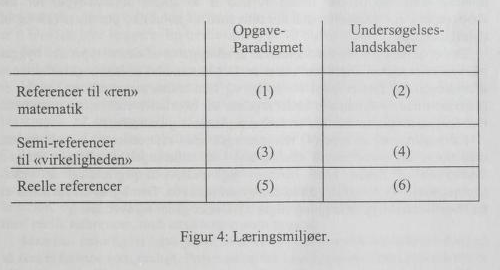
\includegraphics[scale = 0.9]{../figures/laeringsmiljoer.png}
\caption{Kilde: \protect\citeA{skov98}.}
\label{fig:skov98}
\end{figure}

\end{document}
